% -*- latex -*-
% FILE: "/home/evmik/jobs/wm/2011_spring_Analog_Electronics_252/final_exam/questions/matched_njfet_follower.tex"
% LAST MODIFICATION: "Thu, 05 May 2011 10:50:43 -0400 (evmik)"
% (C) 2011 by Eugeniy Mikhailov, <evgmik@gmail.com>
% $Id:$

\question{}
	Consider the circuit shown below. \\
	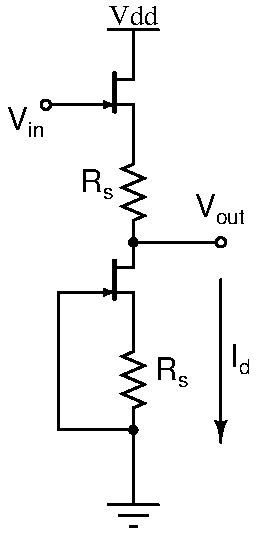
\includegraphics[height=2in]{./schematics/njfet_matched_follower}\\
	NJFETs in this circuit are {\bf  matched}. 
	Presume that $V_{dd}$ is large enough for transistors to be in saturation.
	\begin{parts}
		\part[5]
		First consider only bottom part (below $V_{out}$ terminal). It can be
		thought as a constant current source with current $I_d$ (assume that it
		is somehow known to you).
		
		Write the {\bf symbolical} expression for the $V_{GS}$ of the bottom transistor.
		\vskip .5in
		$V_{GS}=$

		\part[15]
		Using above information. Derive the {\bf symbolical} expression for the output
		voltage  $V_{out}$ in terms of the input voltage, $V_{GS}$, $I_d$,  and
		$R_s$. {\bf Hint:} you might not need all of them at the very end. 
		\vskip 1.8in
		$V_{out}=$

		\part
		The  transistors parameters are the following: the pinch off voltage
		$V_p=-2$~V, the coefficient $k=2\times10^{-3}$~A/(V$^2$). Supply
		voltage $V_{dd}=20$~V, $R_s=500$~$\Omega$. 
		\begin{subparts}
			\subpart[5]
			Find  the quiescent current supplied by the power supply.
			\vskip 1in
			$I_{d}=$

			\subpart[5]
			Find  the quiescent power dissipated by this circuit
			\vskip .5in
			$P_{q}=$
		\end{subparts}

	\end{parts}
	\pagebreak
